\subsection{Question 1}

\lstinputlisting[caption=Matlab Commands,showstringspaces=false,language=Matlab]{../a0_q1.m}

\begin{figure*}[h]
\centering
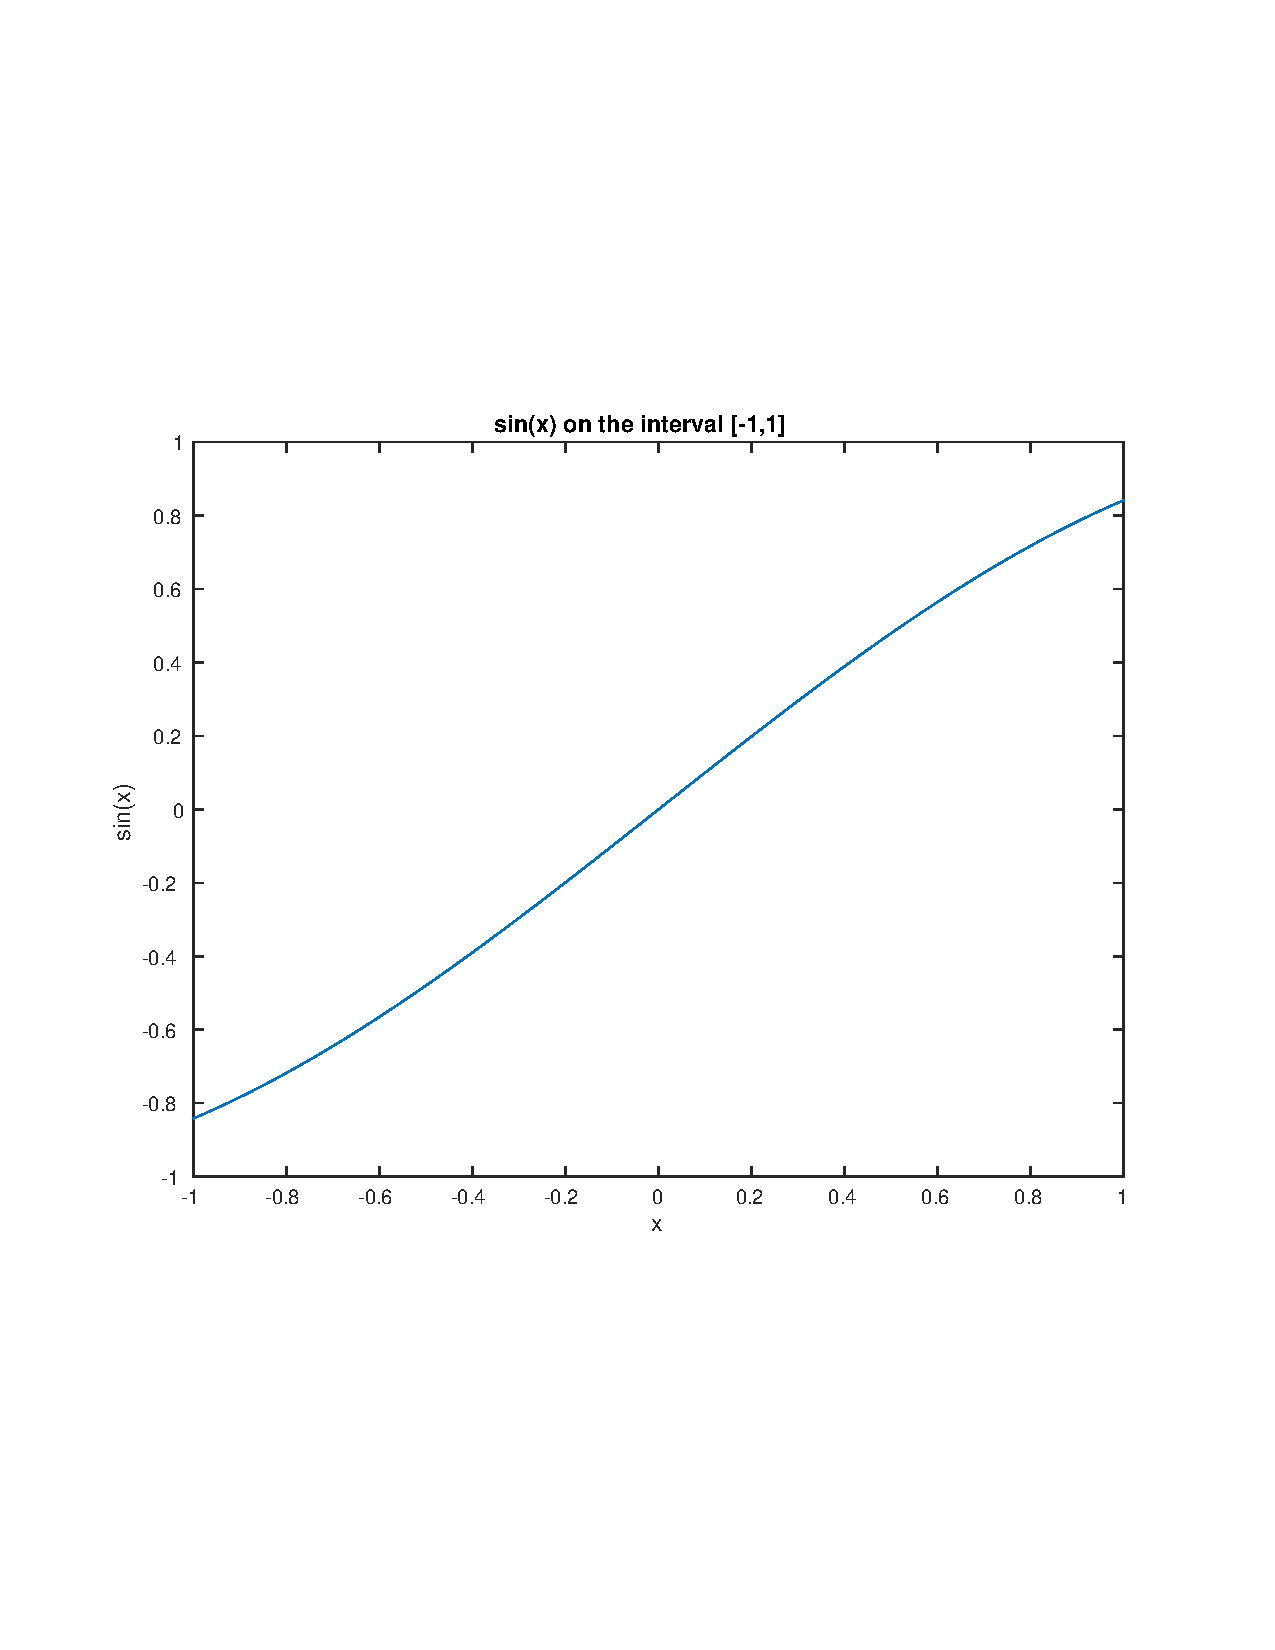
\includegraphics[trim = 20mm 20mm 20mm 20mm, clip, width=.65\textwidth]{figs/a0_q1.pdf}
\label{fig:a0_q1}
\end{figure*}

\newpage
\subsection{Question 2}

\lstinputlisting[caption=Matlab Commands,showstringspaces=false,language=Matlab]{../a0_q2.m}

\begin{equation}
  x = 
  \begin{pmatrix}
    -1.0000 \\
    1.0000 \\
%    \vdots\\
    1.0000 \\    
    1.0000 \\
    1.0000 \\
    1.0000 \\
    1.0000 \\
    1.0000 \\
    1.0000 \\
    1.0000 \\
    1.0000 \\
    1.0000 \\
    1.0000 \\
    1.0000 \\    
    1.0000 \\
    1.0000 \\
    1.0000 \\ 
    1.0000 \\
    1.0000 \\
    -17.0000 
  \end{pmatrix}
\end{equation}

\newpage
\subsection{Question 3}

\lstinputlisting[caption=ssolve functions,showstringspaces=false,language=Matlab]{../ssolve.m}


\newpage
\subsection{Question 4}

\lstinputlisting[caption=Matlab Commands,showstringspaces=false,language=Matlab]{../a0_q4.m}

\newpage
\subsubsection{Part A}

\begin{figure*}[h]
\centering
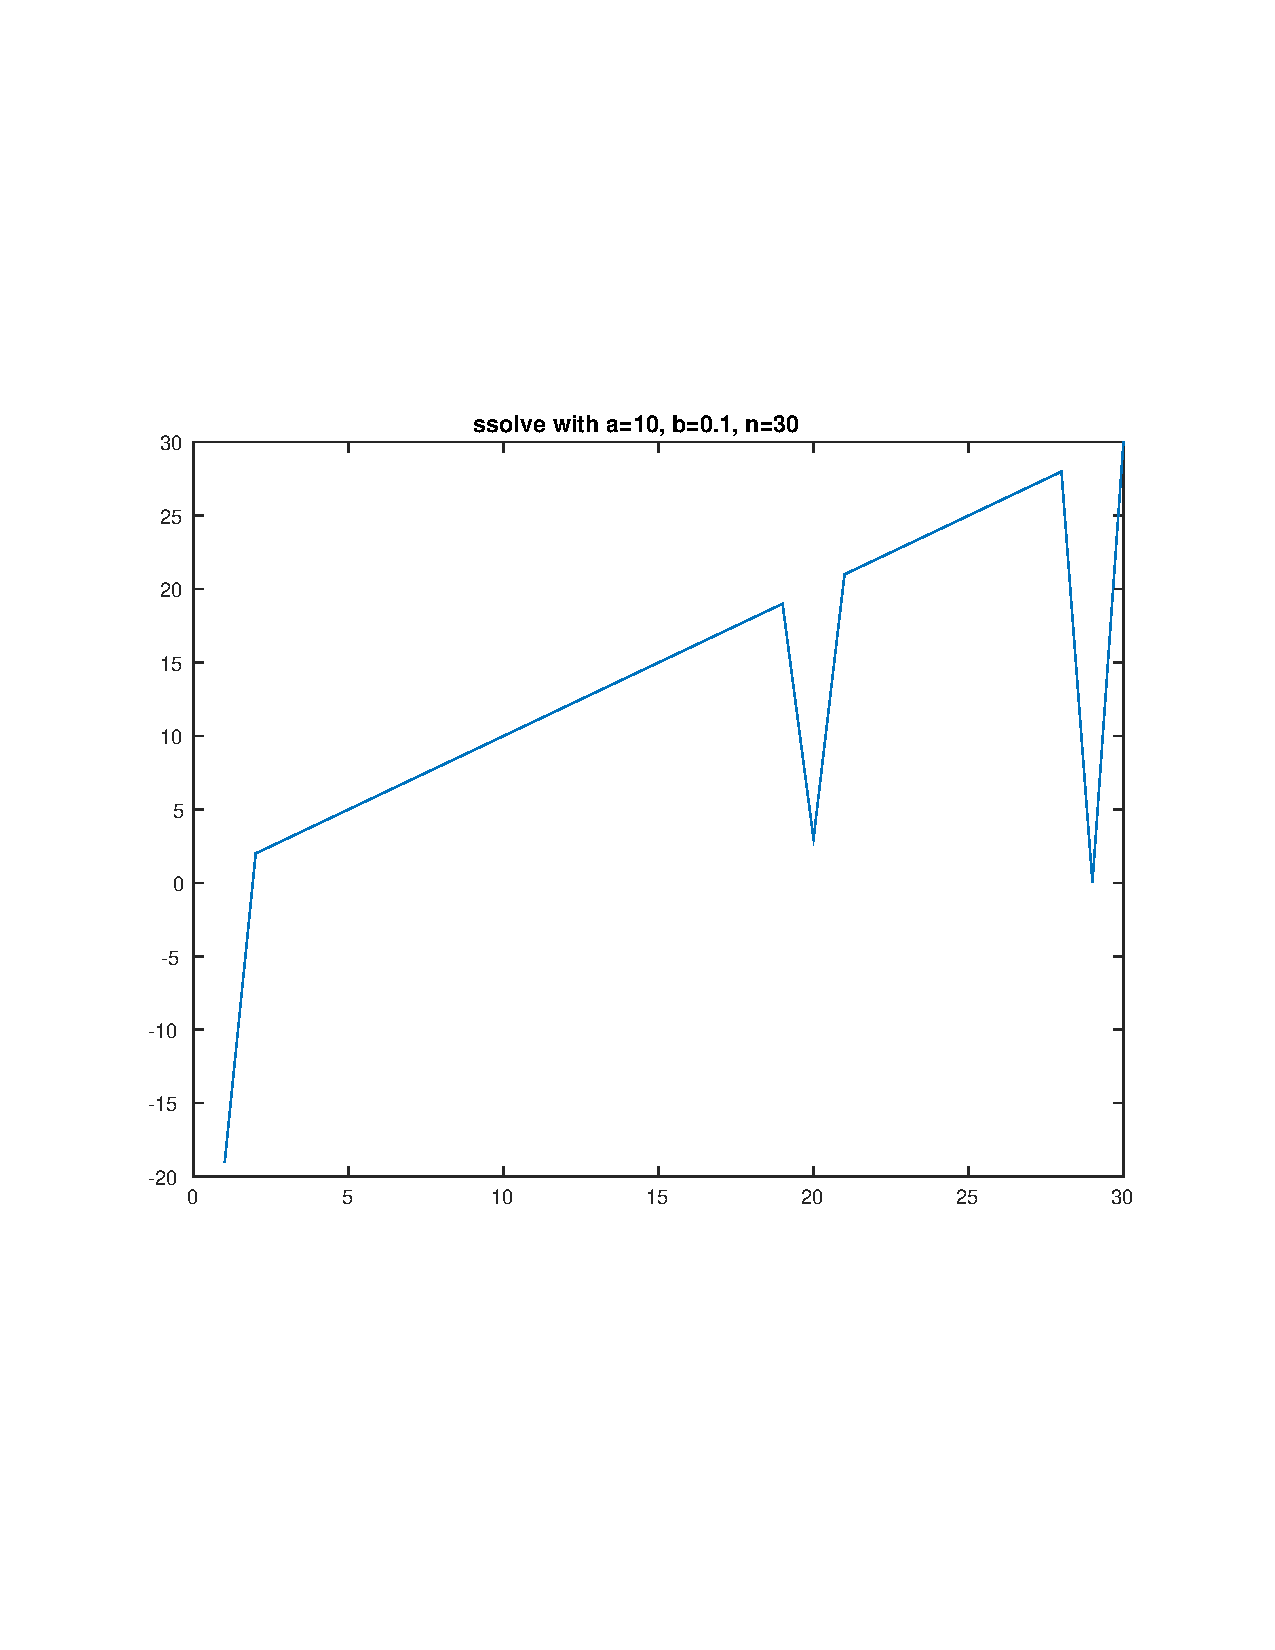
\includegraphics[trim = 20mm 20mm 20mm 20mm, clip, width=.8\textwidth]{figs/a0_q4_a.pdf}
\label{fig:a0_q4_a}
\end{figure*}

\newpage
\subsubsection{Part B}

\begin{figure*}[h]
\centering
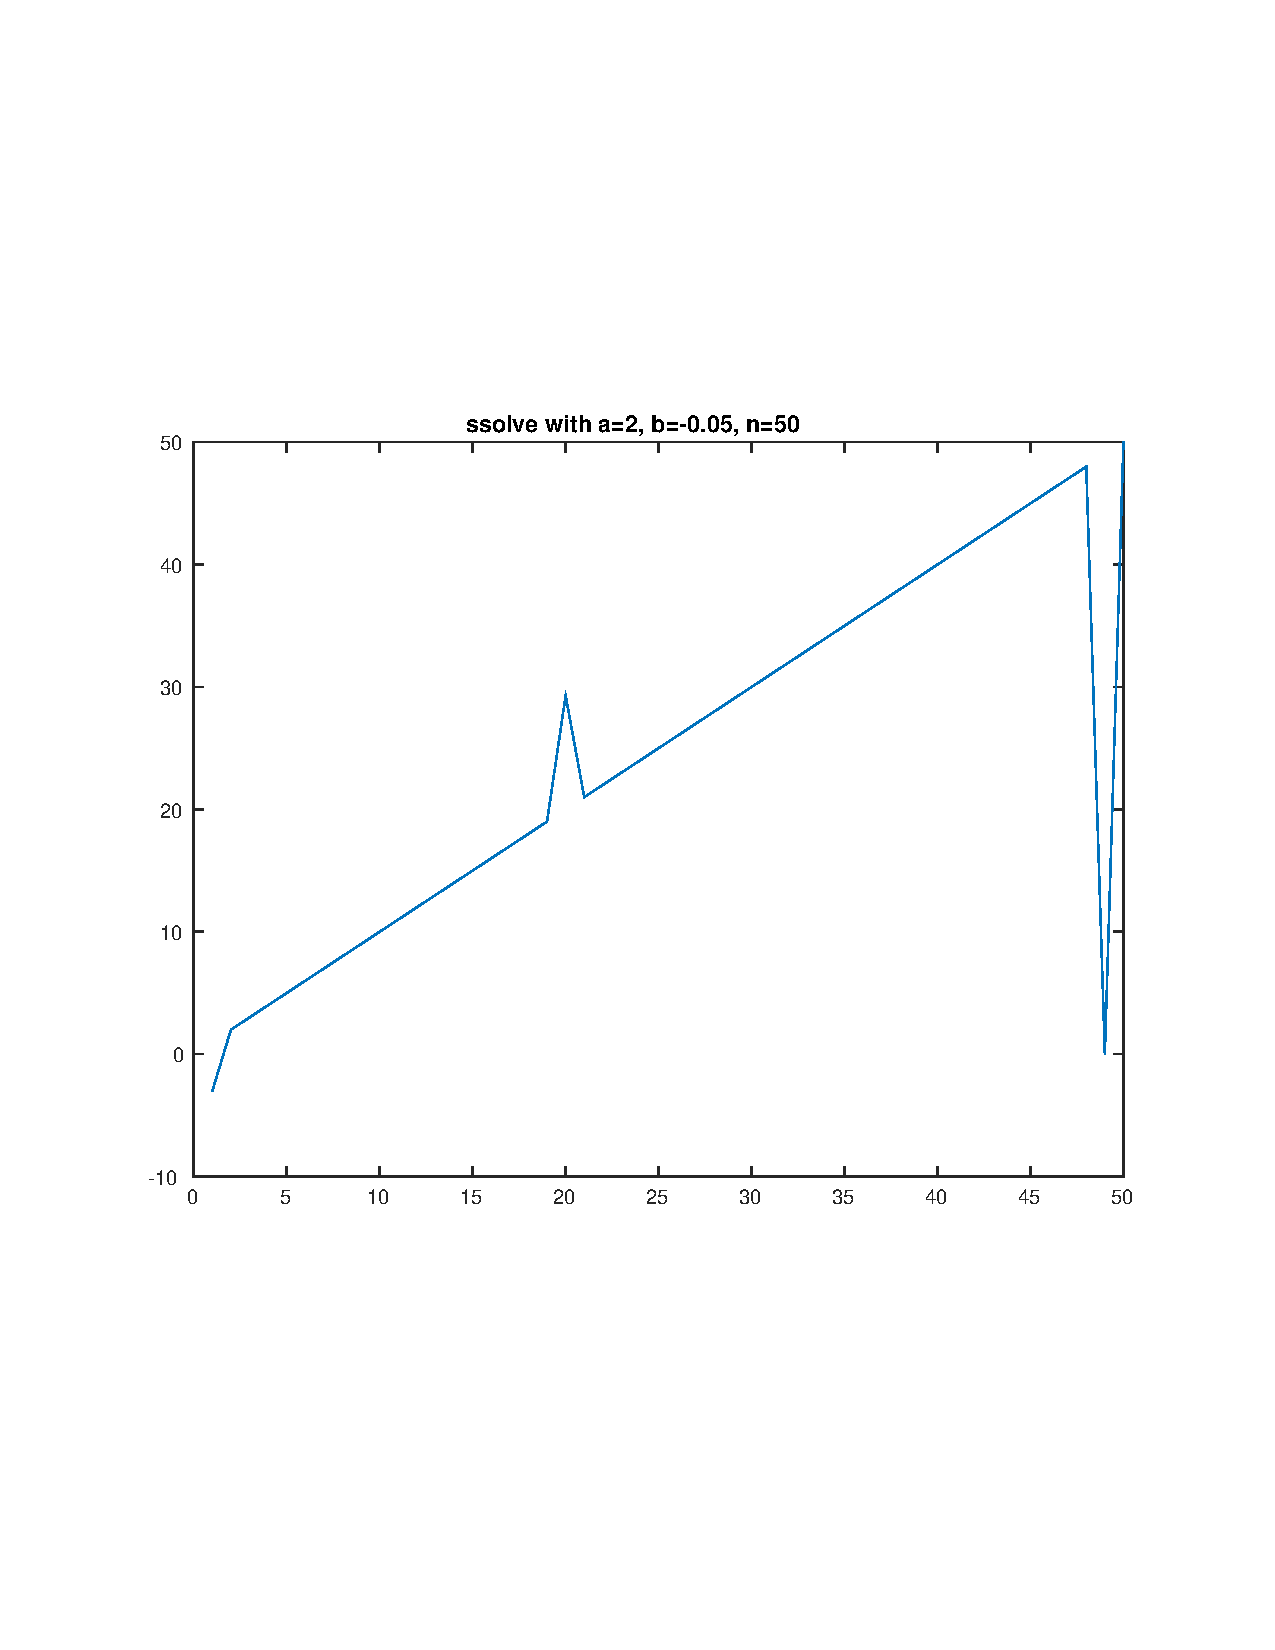
\includegraphics[trim = 20mm 20mm 20mm 20mm, clip, width=.8\textwidth]{figs/a0_q4_b.pdf}
\label{fig:a0_q4_b}
\end{figure*}
